\uuid{UaqF}
\exo7id{5766}
\titre{exo7 5766}
\auteur{rouget}
\organisation{exo7}
\datecreate{2010-10-16}
\isIndication{false}
\isCorrection{true}
\chapitre{Intégration}
\sousChapitre{Intégrale de Riemann dépendant d'un paramètre}
\module{Analyse}
\niveau{L2}
\difficulte{}

\contenu{
\texte{
Pour $x\in\Rr$, on pose $F(x)=\int_{-\pi}^{\pi}\ln(1-2x\cos\theta+x^2)\;d\theta$.
}
\begin{enumerate}
    \item \question{\begin{enumerate}}
\reponse{\begin{enumerate}}
    \item \question{Montrer que $F$ est paire, définie et continue sur $\Rr$, dérivable sur $\Rr\setminus\{-1,1\}$.
Préciser une expression de $F'(x)$ sous forme intégrale.}
\reponse{\textbf{Parité de $F$.} Soit $x$ un réel du domaine de définition de $F$. En posant $t=\theta+\pi$, on obtient

\begin{align*}\ensuremath
F(x)&=\int_{-\pi}^{\pi}\ln(x^2-2x\cos\theta+1)\;d\theta=\int_{0}^{2\pi}\ln(x^2+2x\cos t+1)\;dt\\
 &=\int_{-\pi}^{\pi}\ln(x^2+2x\cos t+1)\;dt\;(\text{par}\;2\pi\text{-périodicité})\\
 &=\int_{-\pi}^{\pi}\ln((-x)^2-2(-x)\cos t+1)\;dt=F(-x).
\end{align*}

Ainsi, pour tout réel $x$, $F(x)$ existe si et seulement si $F(-x)$ existe et de plus $F(x)=F(-x)$.

\begin{center}
\shadowbox{
$F$ est paire.
}
\end{center}

\textbf{Définition de $F$.} Soit $x\in[0,+\infty[$. Pour tout réel $\theta\in[-\pi,\pi]$,

\begin{center}
$x^2-2x\cos\theta+1=(x-\cos\theta)^2+(\sin\theta)^2=\left|x-e^{i\theta}\right|^2\geqslant0$.
\end{center}

De plus, $\left|x-e^{i\theta}\right|=0\Leftrightarrow e^{i\theta}=x\Leftrightarrow x=1\;\text{et}\;\theta=0$. Par suite,

\textbullet~si $x\neq1$, la fonction $\theta\mapsto x^2-2x\cos\theta+1$ est continue sur le segment $[0,\pi]$ et donc intégrable sur ce segment.

\textbullet~si $x=1$, pour tout réel $\theta\in[-\pi,\pi]$ on a $x^2-2x\cos\theta+1=2-2\cos\theta=4\sin^2\frac{\theta}{2}$. La fonction $\theta\mapsto\ln\left(4\sin^2\frac{\theta}{2}\right)$ 

est continue sur $[-\pi,0[\cup]0,\pi]$ et quand $\theta$ tend vers $0$

\begin{center}
$\ln\left(4\sin^2\frac{\theta}{2}\right)=2\ln2+2\ln\left|\sin\frac{\theta}{2}\right|\sim2\ln\left|\frac{\theta}{2}\right|\sim2\ln|\theta|=o\left(\frac{1}{\sqrt{|\theta|}}\right)$.
\end{center}

On en déduit que la fonction $\theta\mapsto\ln\left(4\sin^2\frac{\theta}{2}\right)$ est intégrable sur $[-\pi,\pi]$ et donc que $F(1)$ existe.

Finalement, $F$ est définie sur $[0,+\infty[$ et par parité

\begin{center}
\shadowbox{
$F$ est définie sur $\Rr$.
}
\end{center}

\text{Remarque.} Par parité de la fonction $\theta\mapsto\ln(x^2-2x\cos\theta+1)$, pour tout réel $x$, on a encore $F(x)=2\int_{0}^{\pi}\ln(x^2-2x\cos\theta+1)\;d\theta$.

\textbf{Continuité de $F$.} Soit $A>1$. Soit $\begin{array}[t]{cccc}
\Phi~:&[0,A]\times]0,\pi]&\rightarrow&\Rr\\
 &(x,\theta)&\mapsto&\ln(x^2-2x\cos\theta+1)
\end{array}$.

\textbullet~Pour chaque $x\in[0,A]$, la fonction $\theta\mapsto\Phi(x,\theta)$ est continue par morceaux sur $]0,\pi]$.

\textbullet~Pour chaque $\theta\in]0,\pi]$, la fonction $x\mapsto\Phi(x,\theta)$ est continue par morceaux sur $[0,A]$.

\textbullet~Pour chaque $(x,\theta)\in\Rr^+\times]0,\pi]$, puisque $x^2-2x\cos\theta+1=(x-\cos\theta)^2+(\sin\theta)^2$,

\begin{align*}\ensuremath
|\Phi(x,\theta)|&\leqslant\text{Max}\{\left|\ln(0^2-0\cos\theta+1)\right|,\left|\ln(\cos^2\theta-2\cos\theta\cos\theta+1)\right|,\left|\ln(A^2-2A\cos\theta+1)\right|\}\\
 &=\text{Max}\{2\left|\ln(|\sin\theta|)\right|,\left|\ln(A^2-2A\cos\theta+1)\right|\}=\varphi(\theta).
\end{align*}

On a vu que la fonction $f_1~:~\theta\mapsto2\left|\ln(|\sin\theta|)\right|$ est intégrable sur $]0,\pi]$ et d'autre part, la fonction $f_2~:~\theta\left|\ln(A^2-2A\cos\theta+1)\right|$ est intégrable sur $[0,\pi]$ et donc sur $]0,\pi]$ car continue sur $[0,\pi]$. Puisque $\varphi=\frac{1}{2}(f_1+f_2+|f_1-f_2|)$, on en déduit que la fonction $\varphi$ est continue par morceaux et intégrable sur $]0,\pi]$.

D'après le théorème de continuité des intégrales à paramètres, la fonction $F$ est continue sur $[0,A]$ et ceci pour tout $A>1$. Par suite, la fonction $F$ est continue sur $\Rr^+$ puis par parité,

\begin{center}
\shadowbox{
la fonction $F$ est continue sur $\Rr$.
}
\end{center}
 

\textbf{Dérivabilité de $F$.} Soient $A\in]0,1[$ puis  $\begin{array}[t]{cccc}
\Phi~:&[-A,A]\times[0,\pi]&\rightarrow&\Rr\\
 &(x,\theta)&\mapsto&\ln(x^2-2x\cos\theta+1)
\end{array}$.

\textbullet~Pour chaque $x\in[-A,A]$, la fonction $\theta\mapsto \Phi(x,\theta)$ est continue sur le segment $[0,\pi]$ et donc intégrable sur ce segment.

\textbullet~La fonction $\Phi$ admet sur $[-A,A]\times[0,\pi]$ une dérivée partielle par rapport à sa première variable $x$ définie par

\begin{center}
$\forall(x,\theta)\in[-A,A]\times[0,\pi]$, $\frac{\partial \Phi}{\partial x}(x,\theta)=\frac{2x-2\cos\theta}{x^2-2x\cos\theta+1}$.
\end{center}

De plus,

- pour chaque $x\in[-A,A]$, la fonction $\theta\mapsto\frac{\partial \Phi}{\partial x}(x,\theta)$ est continue par morceaux sur $[0,\pi]$,

- pour chaque $\theta\in[0,\pi]$, la fonction $x\mapsto\frac{\partial \Phi}{\partial x}(x,\theta)$ est continue sur $[-A,A]$,

- pour chaque $(x,\theta)\in[-A,A]\times[0,\pi]$,

\begin{center}
$\left|\frac{\partial \Phi}{\partial x}(x,\theta)\right|=\frac{2|x-\cos\theta|}{|x-e^{i\theta}|^2}\leqslant\frac{4}{|A-1|^2}=\varphi(\theta)$.
\end{center}

La dernière inégalité écrite est claire géométriquement :


$$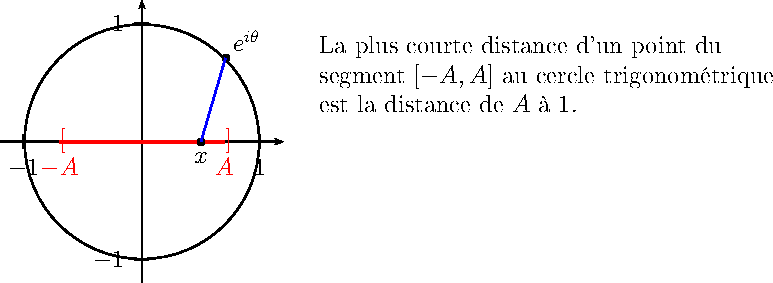
\includegraphics{../images/pdf/UaqF-1.pdf}$$


De plus, la fonction constante $\varphi$ est intégrable sur le segment $[0,\pi]$.

D'après le théorème de dérivation des intégrales à paramètres, la fonction $F$ est de classe $C^1$ sur $[-A,A]$ et sa dérivée s'obtient par dérivation sous le signe somme. Ceci étant vrai pour tout $A\in]0,1[$, $F$ est de classe $C^1$ sur $]-1,1[$ et $\forall x\in]-1,1[$, \rule[-4mm]{0mm}{0mm}$F'(x)=4\int_{0}^{\pi}\frac{x-\cos\theta}{x^2-2x\cos\theta+1}\;d\theta$. La démarche est analogue sur $]-\infty,-1[$ et sur $]1,+\infty[$ et finalement $F$ est de classe $C^1$ sur $\Rr\setminus\{-1,1\}$ et

\begin{center}
\shadowbox{
$\forall x\in\Rr\setminus\{-1,1\}$, $F'(x)=4\int_{0}^{\pi}\frac{x-\cos\theta}{x^2-2x\cos\theta+1}\;d\theta$.
}
\end{center}}
    \item \question{Calculer $F'(x)$.}
\reponse{\textbf{Calcul de $F'(x)$.} Soit $x\in\Rr\setminus\{-1,1\}$. On pose $t=\tan\left(\frac{\theta}{2}\right)$. On a donc $\cos\theta=\frac{1-t^2}{1+t^2}$ et $d\theta=\frac{2dt}{1+t^2}$. On obtient

\begin{align*}\ensuremath
F'(x)&=4\int_{0}^{\pi}\frac{x-\cos\theta}{x^2-2x\cos\theta+1}\;d\theta=8\int_{0}^{+\infty}\frac{x-\frac{1-t^2}{1+t^2}}{x^2-2x\frac{1-t^2}{1+t^2}+1}\frac{dt}{1+t^2}\\
 &=8\int_{0}^{+\infty}\frac{(1+t^2)x-(1-t^2)}{((1+t^2)x^2-2x(1-t^2)+(1+t^2))(1+t^2)}\;dt\\
 &=8\int_{0}^{+\infty}\frac{(x+1)t^2+(x-1)}{((x+1)^2t^2+(x-1)^2)(1+t^2)}\;dt
\end{align*}

Pour tout réel $t$,

\begin{center}
$\left(t^2+\left(\frac{x-1}{x+1}\right)^2\right)(t^2+1)=\left(t-i\frac{x-1}{x+1}\right)\left(t+i\frac{x-1}{x+1}\right)(t-i)(t+i)$.
\end{center}

De plus, $\pm\frac{x-1}{x+1}=\pm1\Leftrightarrow\frac{x-1}{x+1}=-1\Leftrightarrow x=0$.

\textbullet~$F'(0)=4\int_{0}^{\pi}(-\cos\theta)\;d\theta=0$.

\textbullet~Si $x\neq0$, les pôles de la fraction rationnelle $\frac{(x+1)t^2+(x-1)}{((x+1)^2t^2+(x-1)^2)(1+t^2)}$ sont simples et par parité, la décomposition en éléments simples de cette fraction s'écrit

\begin{center}
$\frac{(x+1)t^2+(x-1)}{((x+1)^2t^2+(x-1)^2)(1+t^2)}=\frac{a}{t-i\frac{x-1}{x+1}}-\frac{a}{t+i\frac{x-1}{x+1}}+\frac{b}{t-i}-\frac{b}{t+i}$,
\end{center}

avec

\begin{align*}\ensuremath
a&=\frac{-(x+1)\left(\frac{x-1}{x+1}\right)^2+(x-1)}{(x+1)^2\left(2i\frac{x-1}{x+1}\right)\left(1-\left(\frac{x-1}{x+1}\right)^2\right)}=\frac{-(x+1)(x-1)^2+(x-1)(x+1)^2}{2i(x+1)(x-1)((x+1)^2-(x-1)^2)}\\
 &=\frac{2(x^2-1)}{2i(x^2-1)(4x)}=\frac{1}{4ix},
\end{align*}

et

\begin{center}
$b=\frac{-(x+1)+(x-1)}{2i(-(x+1)^2+(x-1)^2)}=\frac{1}{4ix}$.
\end{center}

Donc

\begin{align*}\ensuremath
8\frac{(x+1)t^2+(x-1)}{((x+1)^2t^2+(x-1)^2)(1+t^2)}&=\frac{2}{ix}\left(\frac{1}{t-i\frac{x-1}{x+1}}-\frac{1}{t+i\frac{x-1}{x+1}}+\frac{1}{t-i}-\frac{1}{t+i}\right)\\
 &=\frac{2}{ix}\left(\frac{2i\frac{x-1}{x+1}}{t^2+\left(\frac{x-1}{x+1}\right)^2}+\frac{2i}{t^2+1}\right)=\frac{4}{x}\left(\frac{x^2-1}{(x+1)^2t^2+(x-1)^2}+\frac{1}{t^2+1}\right)
\end{align*}

Ensuite, en notant $\varepsilon$ le signe de $\frac{x-1}{x+1}$

\begin{align*}\ensuremath
F'(x)&=\frac{4}{x}\int_{0}^{+\infty}\left(\frac{x^2-1}{(x+1)^2t^2+(x-1)^2}+\frac{1}{t^2+1}\right)\;dt\\
 &=\frac{4}{x}\left[\frac{x^2-1}{(x+1)^2}\frac{1}{\frac{x-1}{x+1}}\Arctan\left(\frac{t}{\frac{x-1}{x+1}}\right)\right]_0^{+\infty}=\frac{4}{x}\left(\varepsilon+1\right)\frac{\pi}{2}
\end{align*}

Par suite, si $x\in]-1,1[$, $F'(x)=0$ et si $x\in]-\infty,-1[\cup]1,+\infty[$, $F'(x)=\frac{4\pi}{x}$.

\begin{center}
\shadowbox{
$\forall x\in\Rr\setminus\{-1,1\}$, $F'(x)=\left\{
\begin{array}{l}
\rule[-2mm]{0mm}{0mm}0\;\text{si}\;x\in]-1,1[\\
\frac{4\pi}{x}\;\text{si}\;x\in]-\infty,-1[\cup]1,+\infty[
\end{array}
\right.$.
}
\end{center}}
    \item \question{Déterminer $\lim_{x \rightarrow +\infty}(F(x)-4\pi\ln x)$.}
\reponse{Soit $x>1$.

\begin{center}
$F(x)-4\pi\ln(x)=\int_{-\pi}^{\pi}\ln(x^2-2x\cos\theta+1)\;d\theta-\int_{-\pi}^{\pi}\ln(x^2)\;d\theta=\int_{-\pi}^{\pi}\ln\left(1-\frac{2}{x}\cos\theta+\frac{1}{x^2}\right)\;d\theta=F\left(\frac{1}{x}\right)$.
\end{center}

Par suite, $\lim_{x \rightarrow +\infty}(F(x)-4\pi\ln(x))=\lim_{x \rightarrow +\infty}F\left(\frac{1}{x}\right)=\lim_{y \rightarrow 0}F(y)=F(0)=0$ par continuité de $F$ en $0$.

\begin{center}
\shadowbox{
$\lim_{x \rightarrow +\infty}(F(x)-4\pi\ln(x))=0$.
}
\end{center}}
    \item \question{En déduire $F(x)$ pour tout réel $x$.}
\reponse{\textbullet~$F$ est continue sur $[-1,1]$, dérivable sur $]-1,1[$ de dérivée nulle sur $]-1,1[$. Donc la fonction $F$ est constante sur l'intervalle $[-1,1]$. Par suite, pour tout réel $x\in[-1,1]$, $F(x)=F(0)=0$.

\textbullet~$F$ est dérivable sur $]1,+\infty[$ et $\forall x>1$, $F'(x)=\frac{4\pi}{x}$. Donc il existe $C\in\Rr$ tel que $\forall x>1$, $F(x)=4\pi\ln x+C$ avec $C=\lim_{x \rightarrow +\infty}(F(x)-4\pi\ln x)=0$. Donc $\forall x>1$, $F(x)=4\pi\ln x$.

\textbullet~Si $x<-1$, $F(x)=F(-x)=4\pi\ln(-x)=4\pi\ln|x|$.

\begin{center}
\shadowbox{
$\forall x\in\Rr$, $\int_{-\pi}^{\pi}\ln(x^2-2x\cos\theta+1)\;d\theta=\left\{
\begin{array}{l}
0\;\text{si}\;x\in[-1,1]\\
4\pi\ln(|x|)\;\text{si}\;x\in]-\infty,-1[\cup]1,+\infty[
\end{array}
\right.$.
}
\end{center}}
\end{enumerate}
}
